\chapter{Project Implementation}

\label{ch:fslayout}

In this chapter we'll get into implementation details, extending the solution described earlier in this paper. We'll be presenting the file system layout and how an user can view and create versioned content. The concurrency model and how the content is fetch from remote repositories and merged, will be also presented in the chapters below.

\section{File System layout}
When mounting gitfs, a bare repository and a mount point need to be specified. Gitfs will maintain a local copy of the repository by cloning it into a defined path, named as 'repo\_path'. By default, the location of this cloned repository is set to '\/var\/lib\/gitfs'. Here, gitfs will create a new directory, obtaining it's name from the path (can also be an URL) to the bare repository. One can override this default behaviour and specify an absolute path in which the repository should be cloned, using '-o repo\_path=\/absolute\/path\/'. Gitfs uses the git's objects of this local repository in order to retrieve its content and manage all versioning operations. It can clone local, non-bare repositories, but it doesn't support pushing changes to them. For now, it know to follow only one branch and if no branch is specified, when mounting, it will clone only the master branch and follow it.

Once cloned, the content is retrieve from git objects, using pygit2, and presented in the mount point directory through two directories: current and history. The entire file system will have as owner and group the ones from the users which did the mount operation. This behaviour can be overridden, by specifying at mounting under what group and owner should be mounted. 

In current directory the current state of the content, being just a mirror for the cloned repository. Here, all changes will became commits in the git repository and will get synchronized with the remote. The second directory it's called history, a pretty intuitive name. This directory contains $n$ other directories, one for each day in which a change was made, and those directories will contain $m$ other directories, one for each change in that day. This means that the entire number of directories in the history directory is $n*k (k \in \mathcal{N}, 0<k<m+1)$, each one of them representing a state in which the repository's content was at a certain time.

\begin{figure}[h]
  \begin{center}
    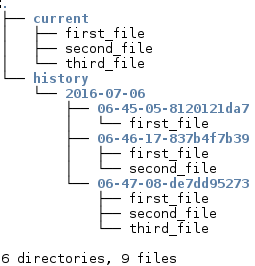
\includegraphics[width=10cm]{layout/gitfs_layout.png}
  \end{center}
\end{figure}

The current and history directories are virtual directories which does not exists on disk. The entire set of operations which are done on current directory are actually performed on the locally cloned repository. Also, in history directory, all those directories are not physical on the storage device. Those directories are created from git objects of local repository. Those objects are only once loaded in memory and cached, and from them, whenever one uses history directory or one of its directories, the content located in those is generated dynamically from the cached git objects.

\section{Views}
In order to better explain how gitfs manage the content in those directories and file system's operations, we can make a parallel example with how an HTTP service handles the requests. 

The entire file system layout can be translated into URLs. Each path in the file system can be viewed as an URL, being part of an HTTP service. When a request is made on a certain URL, a handler will be trigger and a response will be returned. The request can be made with different HTTP methods: GET, POST, PUT, DELETE etc. For each of those methods the request handler can respond with different content. When a client requests the content from a certain URL it will use GET. When it wants to change it, it usually uses POST, but in order to differentiate the type of the change, other methods can be used (PUT, DELETE or PATCH). The request handler can act like a proxy to other parts of the application will do the actual work, returning a response to the request handler which will returned it back to the client.

Those parts of the application which implement the business logic are usually called controllers, in a MVC (Model View Controller) framework. Other parts from a MVC framework are: Model (contains logic which deals with data manipulation) and Views (those components are what the client actually see). Traditionally, the Controller serves as a proxy for data, from Model to View. In a modern MVC architecture the business logic can be placed in an intermediary layer, between Models and Controllers, or directly in Models. Having multiple controllers, the request handler needs to decide which controller to instantiate and use, for which URL. A solution to this problem will be to route the request using some predefined routing rules. Those rules can be described using regular expressions. Because the of a request handler is to route the request to a controller, we'll be calling it Router.

As one can observe, this behave can applied very easily to a FUSE based file system. In order to develop a FUSE file system one needs to implement an interface which represents the set of operations which can be performed on that file system. To be more specific, fusepy offers you a base class, called 'Operations', which acts like an interface (but in Python, being weakly type, it doesn't provide the concept of interfaces). You need to inherit from that class and implement a set of methods which represents the set of operations supported by the file system (read, write, open, close, mkdir etc.).

Because all those method will have a pathname as argument, we can use the model described earlier, inspired by the MVC pattern. The paths to different files or directories can be viewed as URLs and a performing operation as an HTTP request. We can implement different controllers, for different paths and use a router to route a certain operation to a controller.

This idea came originally from Django (a popular Pyhon based web framework) which implements a variation of MVC called MVT (Model-View-Template). In this pattern, the View actually represents the controller and the Template will be the View (a little bit confusing). That's why, in this implementation, the Views are actually Controllers.

For each directory from the mount point we implemented a series of views: CommitView, HistoryView, IndexView and CurrentView. In order to reuse common logic we used two classes:

\begin{itemize}
    \item PassthroughView - a view which doesn't change the behaviour of the file system. It's implemented as a blind proxy to the actual kernel file system, by calling, for each operation, the corresponding system call.
    \item ReadOnlyView - used to restrict the access to any write operation. If a user space application will want to invoke a write operation, an EROFS will be raised.
\end{itemize}

Those views are inherited by the actual, user facing, views:
\begin{itemize}
    \item PassthroughView
    \begin{itemize}
        \item CurrentView – is the view which handles the current directory. It is a PassthroughView meaning that all operations will be executed by an individual file system, without changing the outcome. This view is also responsible for managing the changes and initiate the commit process.
    \end{itemize}
    
    \item ReadOnlyView
    \begin{itemize}
        \item HistoryView – view which handles the history directory and group commits by day. Also, it handles the history/{day} directories. Using the git objects from previously cloned repository, it can retrieve when changes occured and using a hashmap it can group them by day.
        \item CommitView – is the view which handles the history/*day*/*commit* directories. In a such give directory is represented a snapshot of the repository, when a certain change was made, in a certain day. This behaviour can be used to retrieve content, from an earlier version, but in a more tangible why, without to use any commands. CommitView is read-only because you are not allowed to change the history. In order to restore a file to an older state you need to copy it from one of those kind of directories and put it in the current directory.
        \item IndexView – is the view which handles the directory represented as mount point. It's responsible only by current and history directory and doesn't implement any custom logic.
    \end{itemize}
\end{itemize}

All those views inherit from a base class called View. The View class has the purpose of mixing the Operations and LogginMixin classes from fusepy. Beside that, it also offer an easy mechanism for attributes initialization. See figure ~\ref{fig:views_diagram} for a better overview of the arhitecture.

\begin{figure}[h]
  \begin{center}
    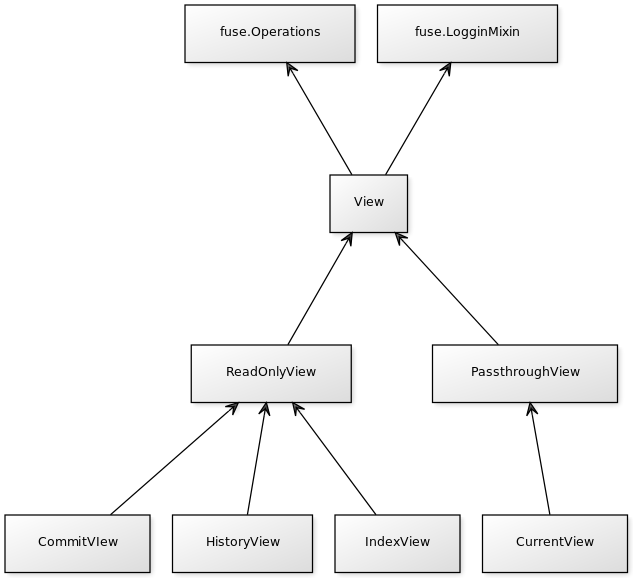
\includegraphics[width=15cm]{concurrency/views-gitfs.png}
  \end{center}
  \caption{Views class diagram}
  \label{fig:views_diagram}
\end{figure}

There is one special component which is not in figure ~\ref{fig:views_diagram}. That component is the Router. In order to implement the routing logic, we need a class which will look a lot like a view. Event if the Router has almost all components of a View, it can't be considered a view, because its purpose is not to implement any file system specific logic, but to act like a proxy for those components which implement.

The Router is the entry point for our file system. When mounting the file system, fusepy will receive as an argument an Operation based class. The Operation class, from fusepy, has some methods which need to be implemented in order to associate a specific behaviour to the file system. In our case, the Route doen't need to do that, it only needs to pretend that will implement the method, but under the hood it will use the methods from specific views.

After the mounting operation is complete, FUSE kernel module, will take care of the operations. For each system call, invoked by an user space application, it will spawn a thread in which will use the object passed to it at mounting and try to call the method which implements the requested operation. Python, being a dynamic and weak typed language, we can intercept this call and inject some custom logic. 

The router receive what operation needs to execute and a path to a certain file. Based on some given regular expression, it determines which view to use. Instead of initializing a new view for each operation, a cache is used. In that cache are stored initialized views, one for each file path that was requested. The cache is implemented as an LRU cache in order have a hard limit on the quantity of memory used by Gitfs. The router will search in that cache, based on a cache key composed by the path of the file, and if the path is in cache, it will return the view associated to it, otherwise it will create a new one and store it in the cache.

Once the view is obtain, the Router will call the specific method which corresponds to the requested operation. A complete example is illustrated in figure ~\ref{fig:routing}.

\begin{figure}[h]
  \begin{center}
    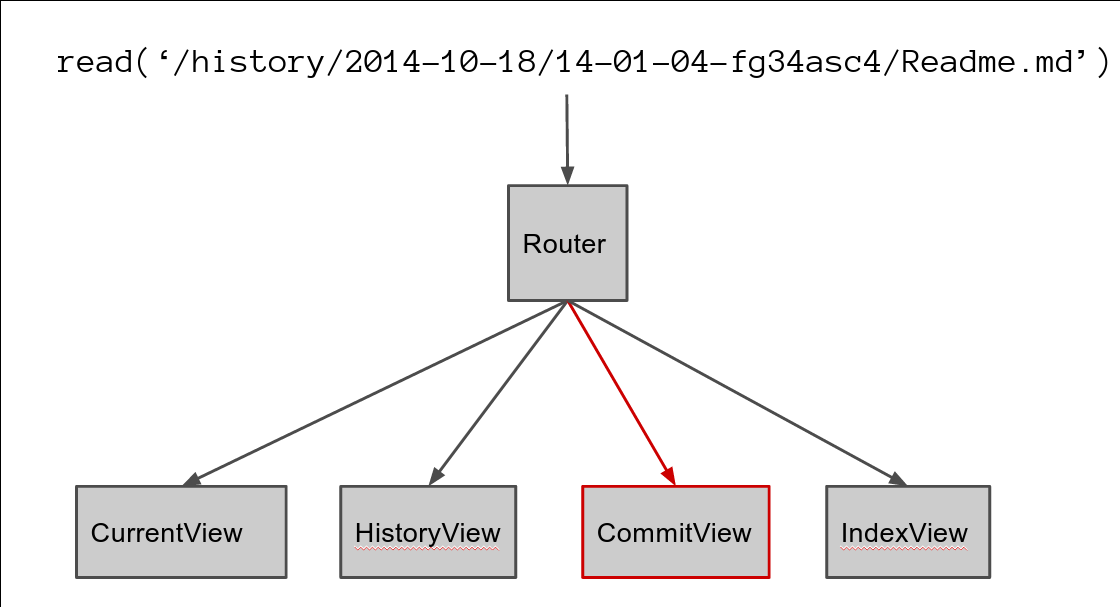
\includegraphics[width=15cm]{layout/router.png}
  \end{center}
  \caption{Operation call flow}
  \label{fig:routing}
\end{figure}

As you can see from the example, when a read system call is used by a user space application, FUSE will trigger a read operation call, using the Router for that. The Router will check if the path is not in the cache. If not, based on regular expressions, will choose to use the CommitView, because the path to the requested file contains a full snapshot description. The Router will also pass some important information to the view, like the name of the requested file and the commit hashed, processed from the path. With those information, the CommitView will be able to retrieve the content for the `Readme.md` file, from the given date. 

\section{Behaviour}

Whenever you will change something in the current directory a commit job will be trigger. Eventually, the job will finish with a commit, and after certain commits were made, they will be pushed to a remote repository. In this way you can be synchronized  with other people whom are working on the same content.

If one of your collaborators already pushed something on the remote, before your pushing, gitfs will try to merge your changes, with the remote one, and in case of conflict, you're changes will have priority. This mechanism it's called: merging with accept mine strategy. Gitfs it's a expendable system and you can implement and use your own merging strategy.

Also, in background, a fetch worker it's fetching changes all the time, at a certain period. If somebody changed something and pushed to the remote repository, you will be able to see those changes in a short period of time.

\section{Special Cases}
If any of any synchronization mechanisms fail (merging, pushing or fetching), the filesystem will enter into a read-only mode, in which you will no be able to do any changes your content until you manually solve those conflicts. This is mechanism it's a safety measure in order to prevent inconsistent states multiple and different across changes.

Another safety mechanism it's an idle mode for fetching. When you don't have any activity on your content for mode then 30 minutes, gitfs will gradually deacrease the amount of time between automatically fetching. This mode prevents staturation of ssh connection on the remote server. 